\documentclass[border={0.1cm 0.1cm 0.1cm 0.1cm}]{standalone}  %E,S,W,N

\usepackage{amssymb}
\usepackage{amsmath}
\usepackage{tikz}

\begin{document}
	
	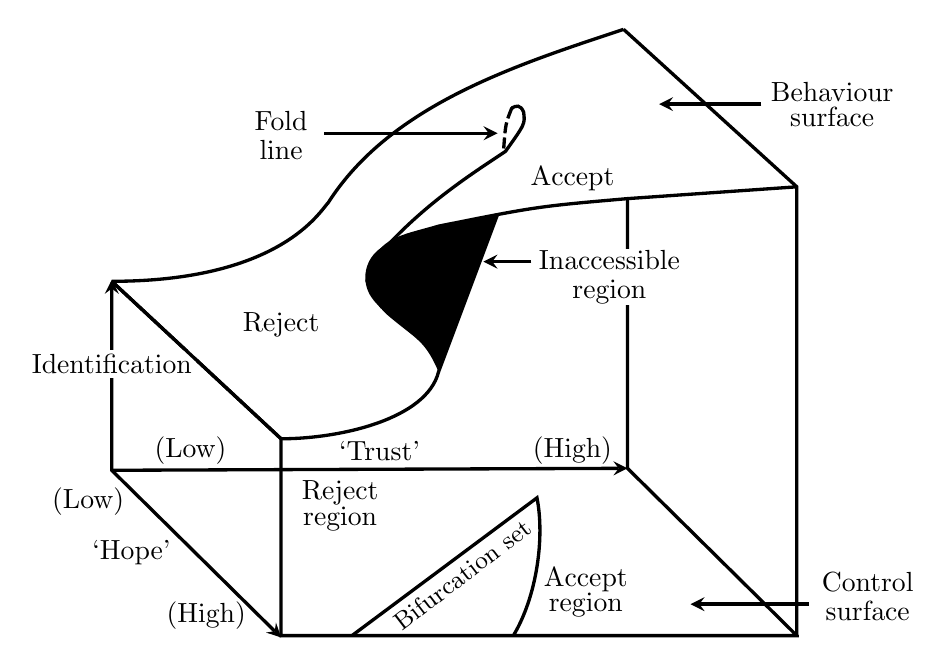
\begin{tikzpicture}[very thick]
	%STRAIGHT LINES
	\draw (-2.15,2)--(0,0)--(0,-2.5)--(6.55,-2.5)--(4.4,-0.375)--(4.4,3.05);
	\draw (6.55,-2.5)--(6.55,3.2)--(4.35,5.2);
	%
	\draw[<->,>=stealth] (0,-2.523)--(-2.15,-0.4)--(-2.15,2.02);
	\draw[->,>=stealth] (-2.15,-0.4)--(4.4,-0.375);
	\draw[white] (6.5927,-2.5+0.04)--(6.5927,-2.5-0.04);
	
	%CURVES
	\draw (-2.15,2) .. controls (0,2) and (0.5,2.9) .. (0.6,3) .. controls (1.4,4.25) and (3,4.75) .. (4.35,5.2);
	\draw (6.55,3.2)--(4.4,3.05) .. controls (3.25,2.95) .. (2,2.7) .. controls (1.5,2.55) and (1.2,2.55) .. (1.1,2);
	\fill (2,0.85)--(2.75,2.85) -- (2,2.7)  .. controls (1.5,2.55) and (1.2,2.55) .. (1.07,2) .. controls (1.25,1.65) .. (1.5,1.45) .. controls (1.75,1.25) and (1.85,1.2) .. (2,0.85);
	\fill (1.52,2.05) circle (0.45cm);
	\draw (1.195,1.77) .. controls (1.23,1.72) .. (1.285,1.668); %kludge
	\draw (2.75,2.85)--(2,0.85) .. controls (1.85,0.25) and (0.75,0) .. (0,0);
	%
	\draw (2.94,4.205) to[bend right] (2.925,4.19);
	\draw (1.3,2.4) .. controls (1.85,3) and (2.4,3.35) .. (2.85,3.65) .. controls (3.1,4) .. (3.08,4.15) .. controls (3.04,4.25) and (2.98,4.23) .. (2.93,4.2);
	\draw[dash pattern=on 4pt off 1.5pt] (2.93,4.2) .. controls (2.85,4) .. (2.825,3.65);
	
	%BIFURCATION SET
	\draw (0.9,-2.5)--(3.25,-0.75) .. controls (3.35,-1.25) and (3.25,-2) .. (2.95,-2.5);
	\node at (2.3,-1.725) {\rotatebox{37.5}{\small Bifurcation set}};
	
	%LABELS
	\node[align=center] at (7.45,-2) {Control \\[-0.5mm] surface};
	\draw[->,>=stealth] (6.7,-2.1)--(5.2,-2.1);
	\node[align=center] at (3.87,-1.95) {Accept \\[-1mm] region};
	\node[align=center] at (0.75,-0.85) {Reject \\[-1mm] region};
	\node at (1.25,-0.15) {`Trust'};
	\node at (3.7,-0.15) {(High)};
	%
	\node at (-1.15,-0.15) {(Low)};
	\node[fill=white,inner sep=1.5] at (-2.15,0.95) {Identification};
		\draw (-2.15,2)--(0,0); %cover up white label
	\node at (-2.45,-0.80) {(Low)};
	\node at (-1.9,-1.45) {`Hope'};
	\node at (-0.95,-2.25) {(High)};
	%
	\node at (0,1.45) {Reject};
	\node[align=center] at (0,3.85) {Fold \\[-0.5mm] line};
	\draw[->,>=stealth] (0.55,3.88)--(2.75,3.88);
	\node at (3.7,3.3) {Accept};
	\node[align=center,fill=white,inner sep=0.4] at (4.17,2.05) {Inaccessible \\[-0.5mm] region};
	\draw[->,>=stealth] (3.18,2.25)--(2.57,2.25);
	\node[align=center] at (7,4.25) {Behaviour \\[-1mm] surface};
	\draw[->,>=stealth] (6.1,4.25)--(4.8,4.25);	
	\end{tikzpicture}
	
\end{document}